\clearpage
\subsection{例題12 動きのある画面を作ってみる}

\subsubsection*{考え方}

変数とpos命令、mes命令などを組み合わせることで、動きのある画面を作ることができます。
ファイル→「開く」メニューから「move.hsp」を読み込んで実行してみましょう。
文字が左からゆっくりと右に移動していきます
変数と計算がどんな役割をしているか考えながら見てください。

\begin{figure}[H]
    \begin{center}
        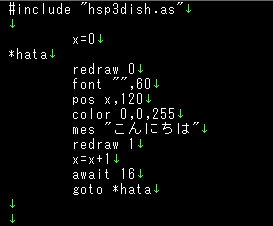
\includegraphics[keepaspectratio,width=8.373cm,height=6.932cm]{text02-img/text02-img050.png}
        \caption{move.hspスクリプトの内容}
    \end{center}
\end{figure}


仕組みがわかったら、次の問題にも挑戦してみましょう。

\begin{itemize}
    \item 文字が動くスピードを変えるにはどうすればいいですか?
    \item 右から左に動かすにはどうすればいいですか?
\end{itemize}

\subsubsection*{例題12 答え}

pos命令のパラメーターに変数が使われています。
つまり、文字を表示する位置を変数で変えられるようにしてあるのです。
変数に代入されている値を増やしたり、減らしたりする計算を覚えておきましょう。

\begin{description}
    \item x = x + 1
\end{description}

という計算は、変数xにきおくされている数字に1を足します。

\begin{figure}[H]
    \begin{center}
        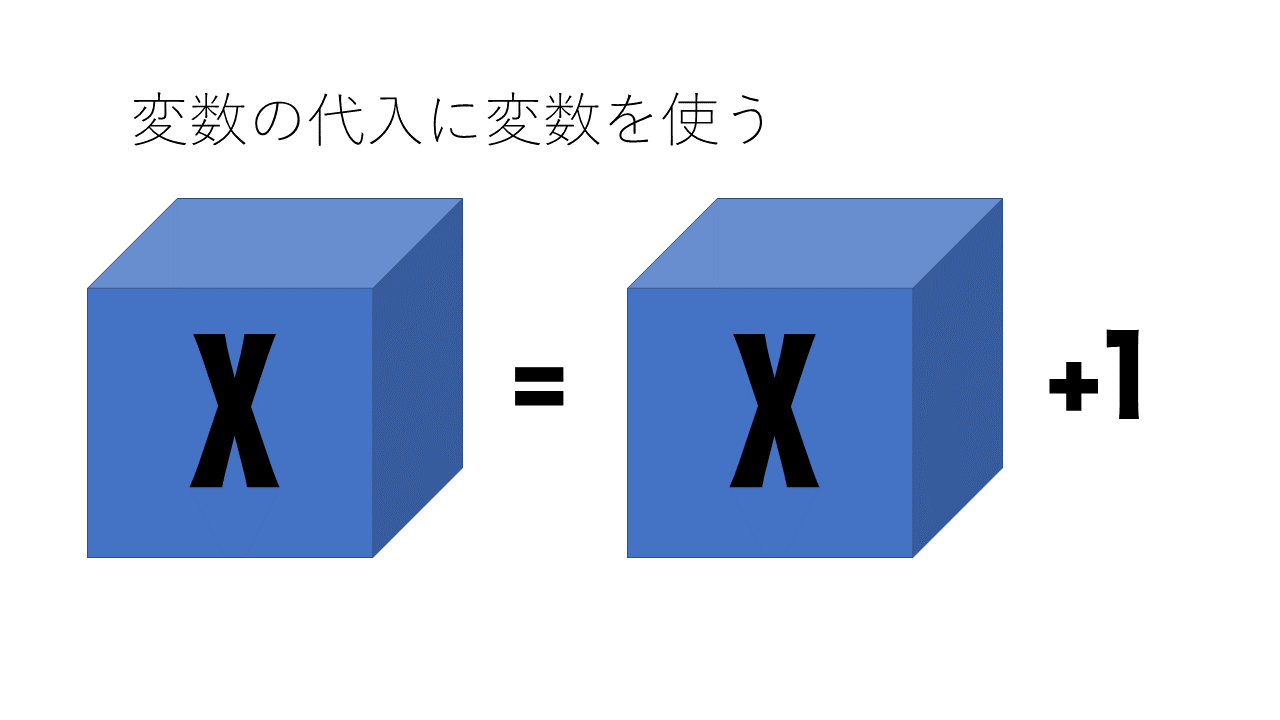
\includegraphics[keepaspectratio,width=10.689cm,height=5.265cm]{text02-img/text02-img051.png}
    \end{center}
\end{figure}

これをくり返すことにより、変数にきおくされている数字で指定された位置を少しずつ変えているのです。
「x=x+1」の「1」を大きな数にすることで、動くスピードを速くすることができます。
文字を右から左に動かすには、変数xの数字を大きい値から、小さい値に減らします。

\begin{description}
    \item x = x + 1
\end{description}

という計算は、変数xにきおくされている数字から1を引きます。
最初に「x=640」として大きな値にしておいて、1ずつ引いていけば右から左に移動するようになるはずです。
実際に試してみて、文字の表示位置が変わったらTAや周りの友達にも見せてあげましょう。

\clearpage
\subsection{例題13 条件判断を自分で使ってみよう}

\subsubsection*{考え方}

条件判断を実際に使ってみましょう。
ファイル→「開く」メニューから「move.hsp」を読み込んでください。
文字が左から右に移動しますが、右まで行ったら、また左に戻るように改造してみましょう。
変数xの値が640を越えたら、0に戻します。
どのように条件判断を書けばいいか考えてみましょう。

条件判断は、if命令を使います。if命令の使い方を思い出してみてください。

\begin{description}
    \item (HSPのルール)
\end{description}

\begin{description}
    \item if命令により条件を判断することができる
    \item ifの後にスペースに続けて条件式を指定します
    \item その後で「:」に続けて条件が正しい時に実行される命令を書きます
\end{description}

\begin{description}
    \item (条件式はいくつか書き方があります)
\end{description}
%修正必要
\ \ \ \ 条件式 \ \ \ \ \ \ \ \ \ 意味

\ \ \ \ {}-{}-{}-{}-{}-{}-{}-{}-{}-{}-{}-{}-{}-{}-{}-{}-{}-{}-{}-{}-{}-{}-{}-{}-{}-{}-{}-{}-{}-{}-{}-{}-{}-{}-{}-{}-{}-{}-{}-{}-{}-{}-{}-{}-{}-{}-{}-{}-{}-{}-{}-{}-

\ \ \ \ 変数名 =
数値\ \ 変数の内容と数値が同じである

\ \ \ \ 変数名 !
数値\ \ 変数の内容と数値が同じではない

\ \ \ \ 変数名 {\textless}
数値\ \ 変数の内容より数値の方が数が大きい

\ \ \ \ 変数名 {\textgreater}
数値\ \ 変数の内容より数値の方が数が小さい

\subsubsection*{例題13 答え}

「もし変数xが640を越えたら、変数xに0を代入する」という命令を書きます。

\begin{description}
    \item if x{\textgreater}640 : x=0
\end{description}

これで、xが1ずつ増えていって、640を越えた時に0に戻す条件判断をしたことになります。

\begin{figure}[H]
    \begin{center}
        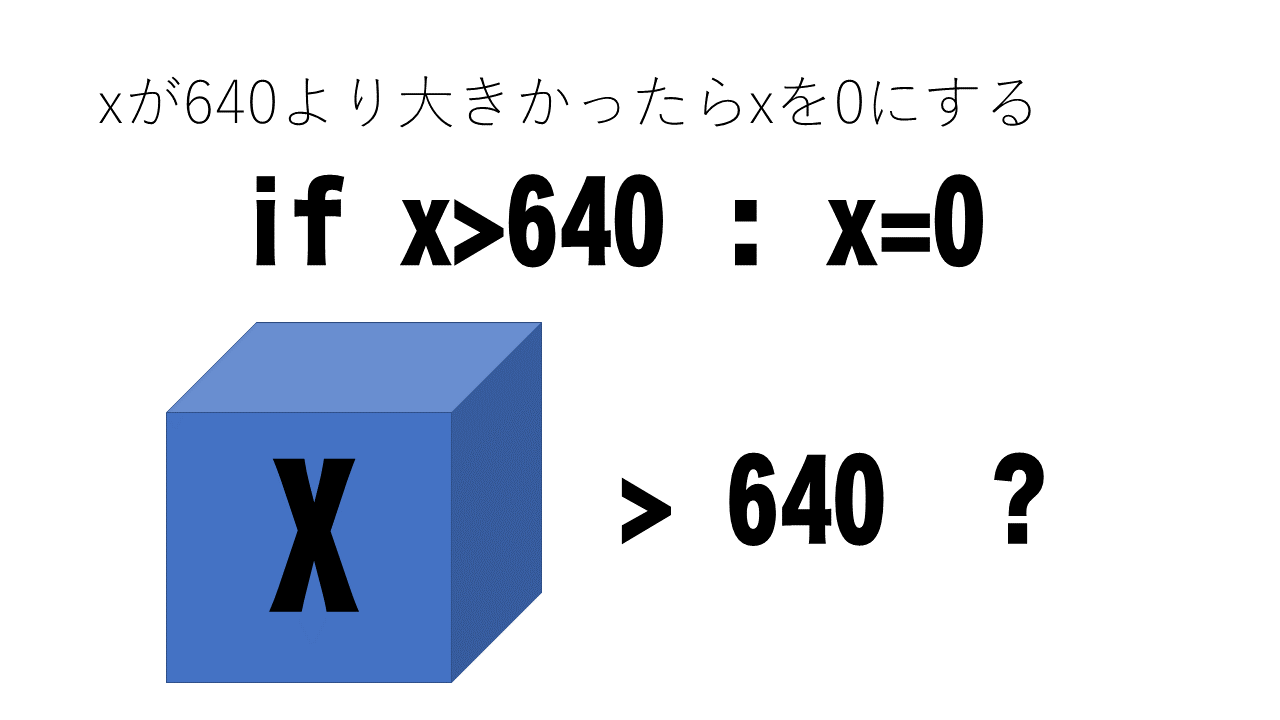
\includegraphics[keepaspectratio,width=11.033cm,height=6.209cm]{text02-img/text02-img052.png}
    \end{center}
\end{figure}

ファイル→「開く」メニューから「handan.hsp」を読み込んでみてください。
実際に試してみて、文字の表示位置が変わったらTAや周りの友達にも見せてあげましょう。

\clearpage
\subsection{例題14 くり返しの方法を知ろう}

\subsubsection*{考え方}

スクリプトは、何度もくり返しができることを習いました。
しかし、時には一定回数だけくり返したいことがあります。そんな時に、すべてまとめて便利に書けるようにしたものがrepeat命令です。
repeat命令の後には、loop命令を必ず書きます。それにより、repeat命令から、loop命令までをすきな回数だけくり返すようになります。
ファイル→「開く」メニューから「repeat.hsp」を読み込んでみましょう。

\begin{description}
    \item repeat 5
    \item gpio 17,1
    \item wait 50
    \item gpio 17,0
    \item wait 50
    \item loop
\end{description}

[F5]キーを押して実行すると、5回だけLEDがてんめつするのがわかります。
「repeat
5」から「loop」までの間を5回くり返したのです。試しに、repeat命令のパラメーターを変更して、5以外の回数になるかどうか試してみましょう。
repeat命令とloop命令の関係について、実際に試しながら学習してみましょう。

\subsubsection*{例題14 答え}

くり返しの回数を変えて色々なパターンを試してみましょう。

\begin{description}
    \item (HSPのルール)
\end{description}

\begin{description}
    \item repeat命令とloop命令は、指定した回数だけくり返しを行う便利な命令
    \item repeatの後にスペースに続けてくり返し回数を書く
    \item loop命令が書かれた場所までを指定した回数くり返す
    \item 回数が0の場合は何も実行しない
    \item 回数を省略(しょうりゃく)した場合は無限にくり返される
\end{description}

実際に試してみて、結果が変わったらTAや周りの友達にも見せてあげましょう。

\clearpage
\subsection{例題15 ポーカーゲームで遊んでみよう}

\subsubsection*{考え方}

実際に変数や乱数が使われているゲームを見てみましょう。トランプを使ったかんたんなゲーム「ポーカーゲーム」を実行します。
ファイル→「開く」メニューから「poker.hsp」を読み込んでください。これはポーカーというトランプのゲームを再現したものです。
最初に配られた5枚のカードから、残しておきたものだけにチェックを付けて、カードを交換します。
できあがった5枚のカードが、きれいな手になっているとコインが増えます。(遊び方がわからない人は、友達や両親、近くの先生に聞いてみましょう)

\subsubsection*{例題15 答え}

変数と計算、条件判断を組み合わせると、このようなゲームが作れます。
まだ難しくで意味がわからないと思いますが、それで問題ありません。
スクリプトを見て、改造できそうな所がないか探してみましょう。
たとえば、コインの枚数はcreditという変数がきおくしています。

\begin{figure}[H]
    \begin{center}
        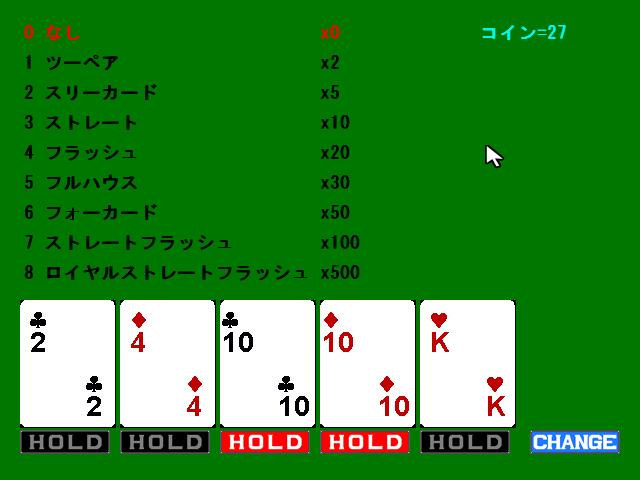
\includegraphics[keepaspectratio,width=10.478cm,height=7.844cm]{text02-img/text02-img053.png}
        \caption{poker.hspの実行画面}
    \end{center}
\end{figure}

\clearpage
\subsection{例題16 スイッチを使ったゲームで遊んでみよう}

\subsubsection*{考え方}

センサーボードのスイッチを使ったゲームに挑戦してみましょう。
ファイル→「開く」メニューから「swjump.hsp」を読み込んでみてください。
スイッチを押してうまくジャンプをして、やってくる柱を避けるゲームです。
いままではキーボードやマウスを使ってゲームをしていましたが、これはセンサーボードのスイッチだけしか使いません。

\begin{figure}[H]
    \begin{center}
        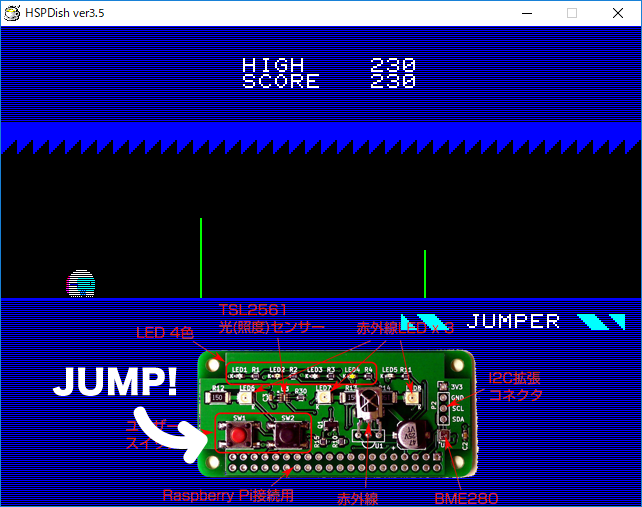
\includegraphics[keepaspectratio,width=8.881cm,height=7.011cm]{text02-img/text02-img054.png}
        \caption{swjump.hspの実行画面}
    \end{center}
\end{figure}

ゲームに慣れてきたら、どこか改造できる所はないか探してみましょう。
センサーボードには、スイッチ以外にも様々なセンサーが内蔵されています。
アイデア次第で色々な応用ができるはずです。
どんなことができるか、あれこれ想像してみてください。自分が作りたいものに向けて、何を覚えればいいのか、何が足りないか考えることもプログラミングでは大切です。

\subsubsection*{例題16 答え}

「swjump.hsp」では色々な変数が使われています。

\begin{description}
    \item score \ 得点をきおくする変数
    \item fps \ \ \ ゲーム全体の速度
    \item barint \ \ ハードルの間隔
    \item levup \ \ \ レベルアップするスコア
\end{description}

これらの値を変えてみると、ゲームの難しさも変わってきます。
色々と変えてみながら、ちょうどいい難しさに改造してみましょう。

\clearpage
\section{ネットでHSPの情報を調べてみよう}

家に帰ってから、インターネットでHSPに関する情報や資料を探すことができます。
HSPは、Raspberry Piだけでなく、Windows PCでも同様に扱うことができます。
家にパソコンやタブレットがある人は、そちらでも活用してみてください。
次のようなページから調べ始めるといいでしょう。(「HSP プログラミング」や「HSP3」などのキーワードでも検索してみましょう)

HSPの情報があるページ

\url{https://hsp.tv/}

HSP講座のあるページ一覧

\url{https://hsp.tv/play/link.html}

HSPプログラムコンテストも開かれています

\url{https://hsp.tv/play/contest.html}

\begin{figure}[H]
    \begin{center}
        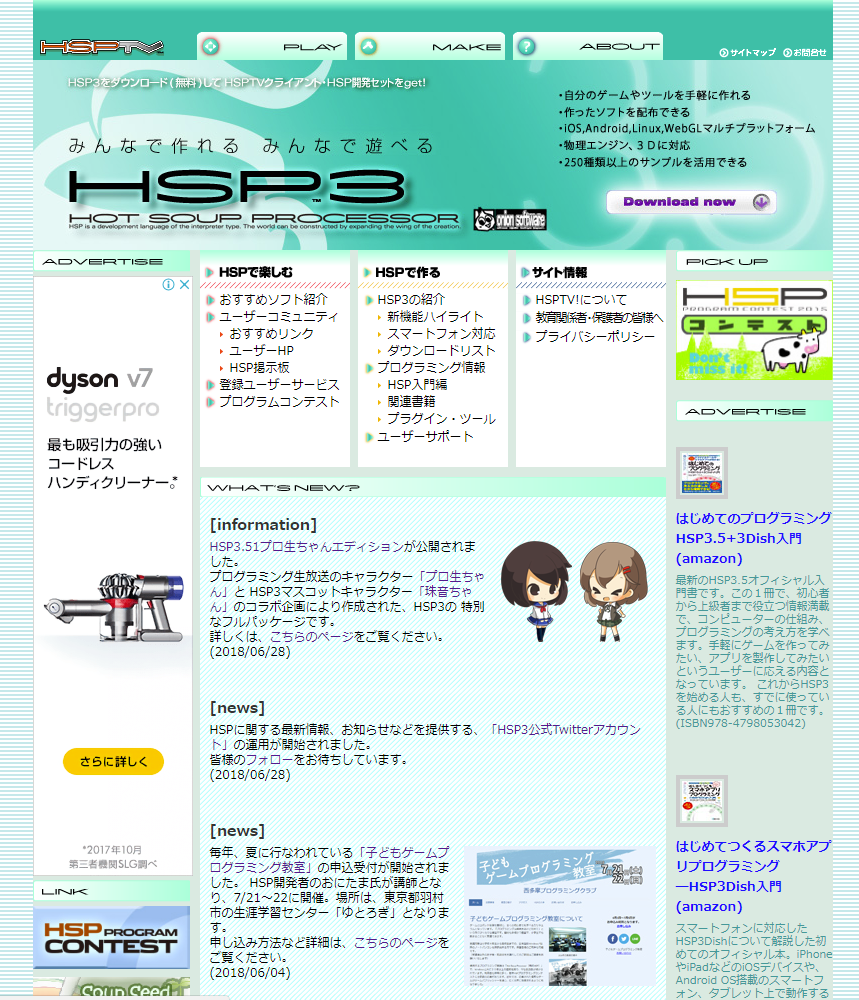
\includegraphics[keepaspectratio,width=9.202cm,height=10.717cm]{text02-img/text02-img055.png}
        \caption{HSP3のホームページ}
    \end{center}
\end{figure}

\clearpage
\section{質問フォーム}

わからないこと、質問したいことがあれば質問フォームから質問しよう!

質問フォームでは、授業でわからなかったことや確認(かくにん)したいことなどをホームページを通して質問できます。たくさん質問してわからないことを解決しよう。

1.
ブラウザで\textbf{授業で使うホームページリスト}を開こう。

\textbf{授業で使うホームページリスト}は/home/ユーザー名/01フォルダの中のlinks.htmlです

リストの4番目の子ども\textbf{IT未来塾質問フォーム}をクリックして開いてください(Figure~\ref{seq:refFigure46})。

\textgt{\bf スマートフォン等からの場合は\url{https://bit.ly/2NHiVgi}を開いてください。}

\begin{figure}[H]
    \begin{center}
        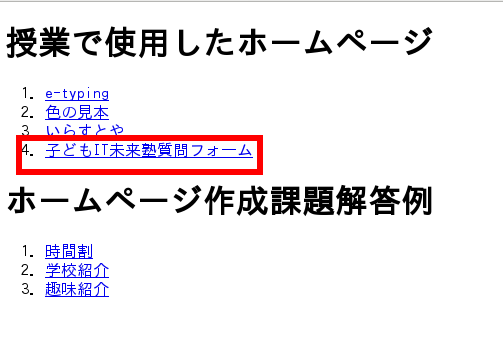
\includegraphics[width=11.231cm,height=7.613cm]{text02-img/textbook-img245.png}
        \caption{ホームページリストより質問フォームを開く}
        \label{seq:refFigure46}
    \end{center}
\end{figure}

2.
質問フォーム(Figure~\ref{seq:refFigure47})が表示されます

\begin{figure}[H]
    \begin{center}
        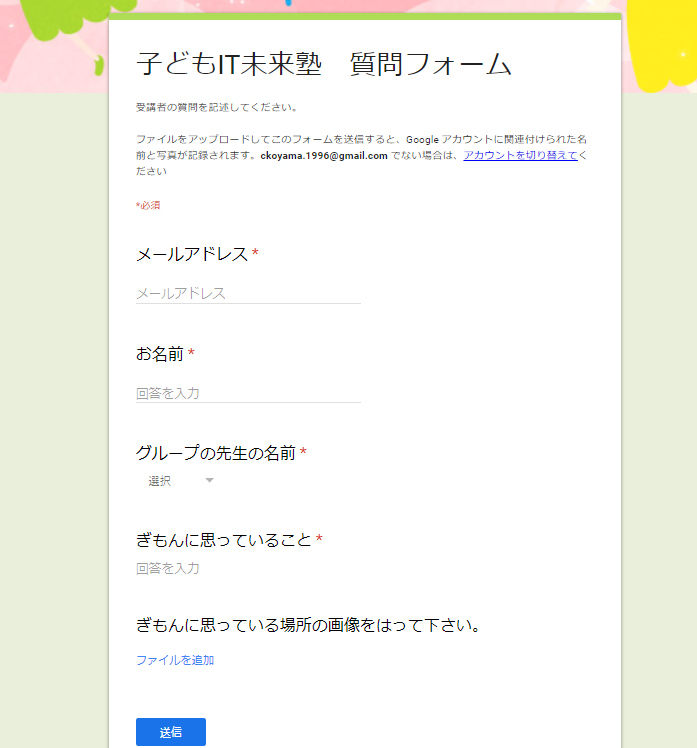
\includegraphics[width=13.263cm,height=14.233cm]{text02-img/textbook-img246.png}
        \caption{質問フォーム}
        \label{seq:refFigure47}
    \end{center}
\end{figure}

メールアドレス、お名前、グループの先生の名前、ぎもんに思っていることを入力します。必要に応じて、ぎもんに思っている場所の画像を追加してください。

\textgt{\bf 送信\textmd{を押すと質問ができます。Figure~\ref{seq:refFigure48}の画面が出たら質問は完了です。}}

\begin{figure}[H]
    \begin{center}
        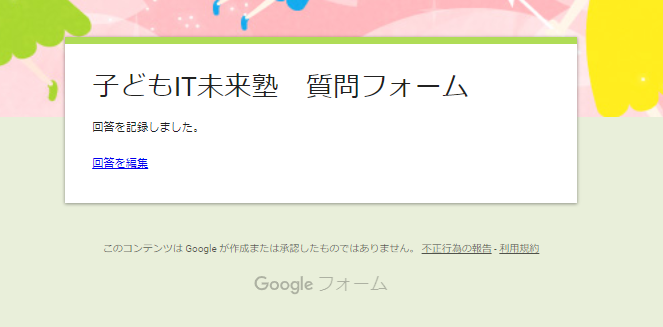
\includegraphics[width=8.871cm,height=4.374cm]{text02-img/textbook-img247.png}
        \caption{質問送信画面}
        \label{seq:refFigure48}
    \end{center}
\end{figure}

メールアドレスのらんに入力したアドレスへグループの先生から回答メールがきます。
メールが来るまで、しばらくお待ちください。数日かかる場合があります。